\section{Experimental Setup}
\label{sec:experiments}

\subsection{Problem Instance and Route Generation}

We construct a 30--40-node tactical delivery graph representing a realistic urban environment with battery constraints, payload limits, and regulatory no-fly zones. Using the soft-max route generator described in Section~\ref{sec:problem}, we produce $N = 2\,048$ feasible candidate routes, each fully respecting battery capacity constraints of $B_{\max} = 80\,\text{Wh}$ with recharge rate $20\,\text{Wh/min}$, payload limits of $Q_{\max} = 5\,\text{kg}$ per drone, wave scheduling across 4 discrete launch windows with inter-wave charging capabilities, and no-fly constraints embedded in the graph adjacency structure.

The combinatorial decision space contains ${2\,048 \choose 10} \times 4^{10} \approx 2.6 \times 10^{26}$ possibilities, encoded using $\lceil\log_2 2048\rceil + \lceil\log_2 4\rceil = 13$ qubits via index representation.

\begin{figure}
    \centering
    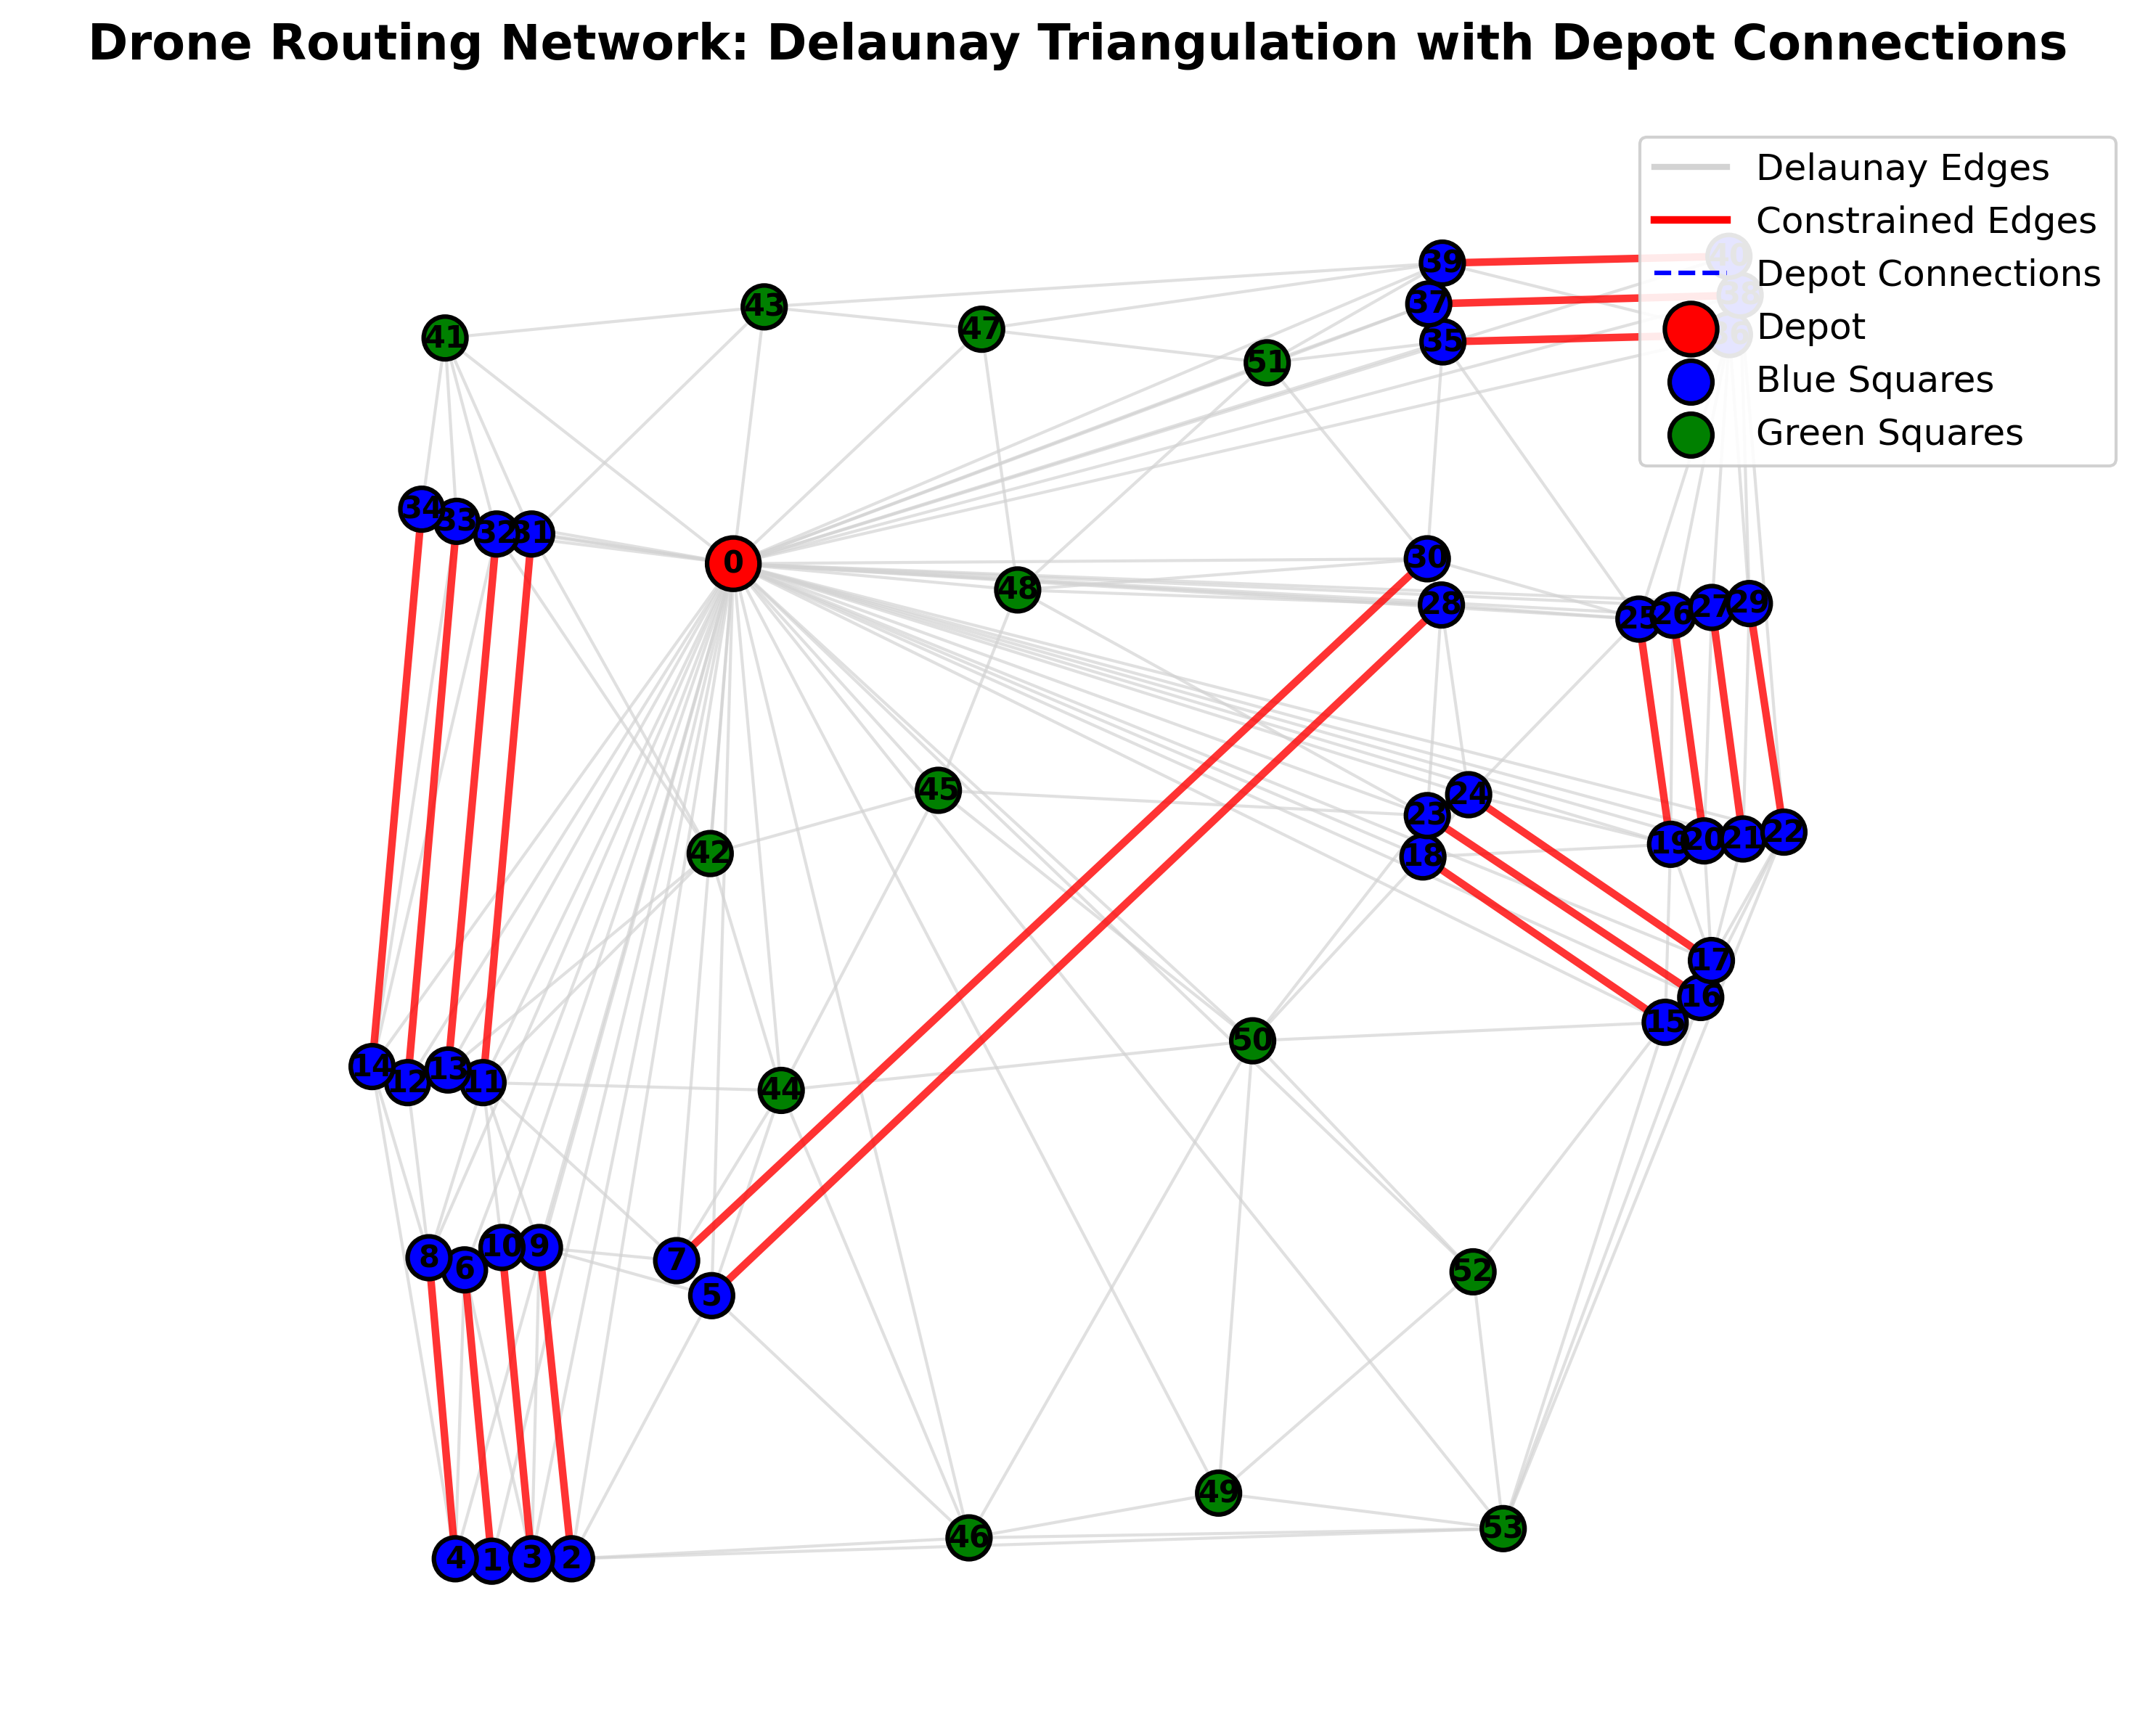
\includegraphics[width=0.8]{figures/graph_simple.png}
    \caption{Graph of study of a realistic drone mission graph adapted from \cite{davies_quantum_2024}, green nodes are customer nodes, while blue nodes also have constrained edges that must be flown, for purposes like surveillance missions. }
    \label{fig:problem_graph}
\end{figure}
\subsection{Classical Baseline: Genetic Algorithm}

To ensure fair comparison, we establish a rigorously tuned GA baseline using comprehensive hyperparameter optimization. Our GA implementation employs bit-string representation with approximately 130 bits per chromosome, dynamic population sizing based on chromosome length, roulette wheel selection with elitism, two-point crossover, and adaptive mutation probability determined through extensive grid search.

We conduct a systematic mutation probability sweep across $\mu \in \{0.15, 0.18, 0.20, 0.22, 0.25\}$ with 30 independent trials per configuration. Statistical analysis identifies $\mu^* = 0.22$ as optimal, achieving mean cost $8\,493 \pm 420$ over 30 trials.

\subsection{Quantum Pipeline: CVaR-VQE}

\subsubsection{Circuit Architecture}
We employ a hardware-efficient variational ansatz with $L \in \{1, 2\}$ layers, yielding 26--52 trainable parameters for the 13-qubit register. Shallow circuits align with NISQ-era coherence limits while maintaining expressivity for the compressed encoding.

\subsubsection{Risk-Aware Objective}
Rather than optimizing the expectation $\mathbb{E}[C]$, we minimize the Conditional Value-at-Risk cost where the best $\alpha$-percentile of $N$ bitstrings drawn contributes to the objective function \cite{barkoutsos_improving_2020}:
\begin{equation}
    \text{CVaR}_\alpha[C] = \mathbb{E}[C \mid C \geq \text{VaR}_\alpha[C]]
\end{equation}

with $\alpha \in \{0.05, 0.1, 1.0\}$ focusing optimization on best-case tail costs. This approach naturally handles heteroscedastic noise from both quantum shot sampling and Monte Carlo route subset evaluation.

\subsubsection{Bayesian Optimization}
We employ Optuna's Aggressive TPE sampler configured with \texttt{prior\_weight = 0.5} for aggressive exploration, \texttt{n\_ei\_candidates = 36} for broad search, and \texttt{MedianPruner} with 90\% retention. This configuration emerged from systematic comparison against Default-TPE and Random sampling across multiple trial budgets, as detailed in Appendix~\ref{sec:appendix_parameters}.

\subsection{Evaluation Protocol}

\textit{Budget Fairness}
All methods receive identical computational budgets of 200,000 objective function evaluations. The noiseless VQE configuration uses 200 iterations with 1,000 samples at 10,000 shots each, while the noisy VQE employs 100 iterations with 1,000 samples at 10,000 shots each. The GA baseline operates with 2,000 population size across 100 iterations. This allocation represents a small fraction of the $O(10^{26})$ search space while ensuring fair comparison across all methods.

\textit{Trial size} Each configuration undergoes 30 independent trials with different random seeds to ensure statistical significance. We report both best-case performance and mean $\pm$ standard deviation across trials to provide comprehensive performance assessment.

\textit{Noise Modeling} To validate practical deployability, we evaluate performance under realistic quantum noise using IBM's calibrated \texttt{ibm\_fez} noise model. The study comprehensively covers circuit depths $L \in \{1, 2\}$, risk parameters $\alpha \in \{0.05, 0.1, 1.0\}$, optimizer comparisons between Aggressive-TPE, Default-TPE, and Random sampling, with 30 trials per configuration ensuring robust statistical analysis. Noiseless baselines use identical hyperparameters, enabling direct measurement of noise-induced performance degradation.